\chapter{Analysis of results}
\label{chapter: analysis of results}








%----------------------------------------- PART 1 --------------------------------------------------

\section{Part 1: SAT verification of the parking configuration}

\subsection{Resolution and analysis of test cases}

\paragraph{}
Here it is a simple description of what each test case attempts to prove:
\begin{itemize}
  \item Case 1 proves the program finds unsatisfiable parking configuration; only one blocked car should suffice to make the configuration unsatisfiable. Car A1 is clearly blocked, so the problem is unsatisfiable. The program reports this as expected.
  \item Case 2 shows a satisfiable parking configuration. No cars are blocked in this case. The program reports this as expected.
  \item The rest of test cases show how the problem \textit{scales} in terms of execution time.
\end{itemize}

\paragraph{}
For tests 3 and above, we have used configurations with increasing number of parking positions, calculated as $M \times N$ (10, 50, 100, 500, 1000, 5000, 10000, 50000, 100000, and 500000). In order to let our computer experiment with more complex problems that require more memory, we have added some extra parameters to \texttt{java} for the \texttt{run.sh} script as follows: \texttt{-XX:-UseGCOverheadLimit -Xmx8000m}.

\paragraph{}
We used a personal computer for getting the execution times. Its technical specifications can be seen on table \ref{tab:computer specs}.
\begin{table}[H]
    \centering
    \rowcolors{2}{gray!25}{white}
    \setlength{\arrayrulewidth}{.1em}
    \setlength\extrarowheight{0.6em}
    \begin{tabular}{M{0.15} M{0.15} M{0.15} M{0.15} M{0.15}}
        \rowcolor{gray!60}
        \hline
        Model & CPU & RAM & Disk & OS\\
        \hline
        Lenovo X270 &
        Intel Core i5-7200U @ 2.50GHz &
        16 GB DDR4 &
        Crucial M300 SSD, 525 GB &
        Ubuntu Studio 16.04 LTS w/ real time kernel\\
        \hline
    \end{tabular}
    \caption{Part 1 benchmark: computer technical specifications}
    \label{tab:computer specs}
\end{table}

\paragraph{}
Figure \ref{fig:part 1 benchmark} shows how the execution time grows with respect to the dimensions of the parking lot.
\begin{figure}[H]
    \caption{Part 1 benchmark: time evolution across different input files}
    \centering
    \label{fig:part 1 benchmark}
    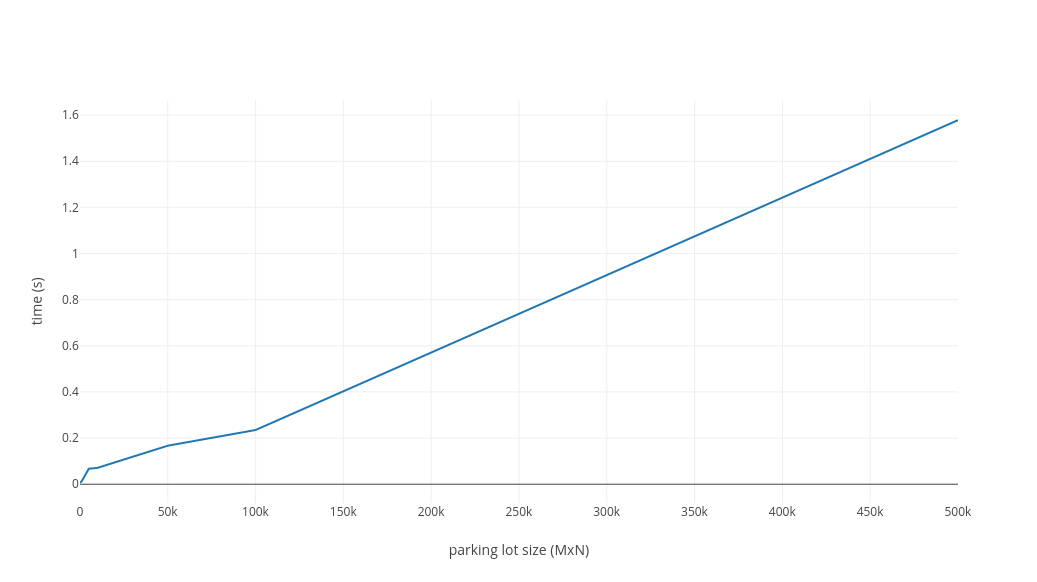
\includegraphics[width=0.7\textwidth]{images/partOneBenchmark}
\end{figure}
This time only measures calls to \texttt{DepthFirstSearch} and \texttt{SimpleSelect} functions from the \texttt{JaCoP} library; that is, it doesn't include the initialization of the boolean variables and literals. We could not finish trying with an input size of 1000000, but it lasted for a considerably larger amount of time compared to previous input sizes before running out of heap space (which had already been expanded with the java arguments we commented before). This difference in execution time with respect to former input sizes makes us think that this problem may follow a close-to-exponential time complexity; that would make sense, since JaCoP uses DFS to look for a satisfiable set of assignments. DFS takes a linear amount of memory, but it uses an exponential amount of time.

%----------------------------------------- PART 2 --------------------------------------------------

\section{Part 2: Heuristic Search}

\subsection{Resolution and analysis of test cases}

\paragraph{}
\warning{Alvaro}{Completar}

\subsection{Comparative analysis of test cases}

\paragraph{}
\warning{Alvaro}{Completar}
